% RGB color mixing
% Author: Henrik Skov Midtiby <http://midtiby.blogspot.com/>
\documentclass{article}
% Set target color model to RGB
\usepackage[rgb]{xcolor}
\usepackage{tikz}
\begin{document}

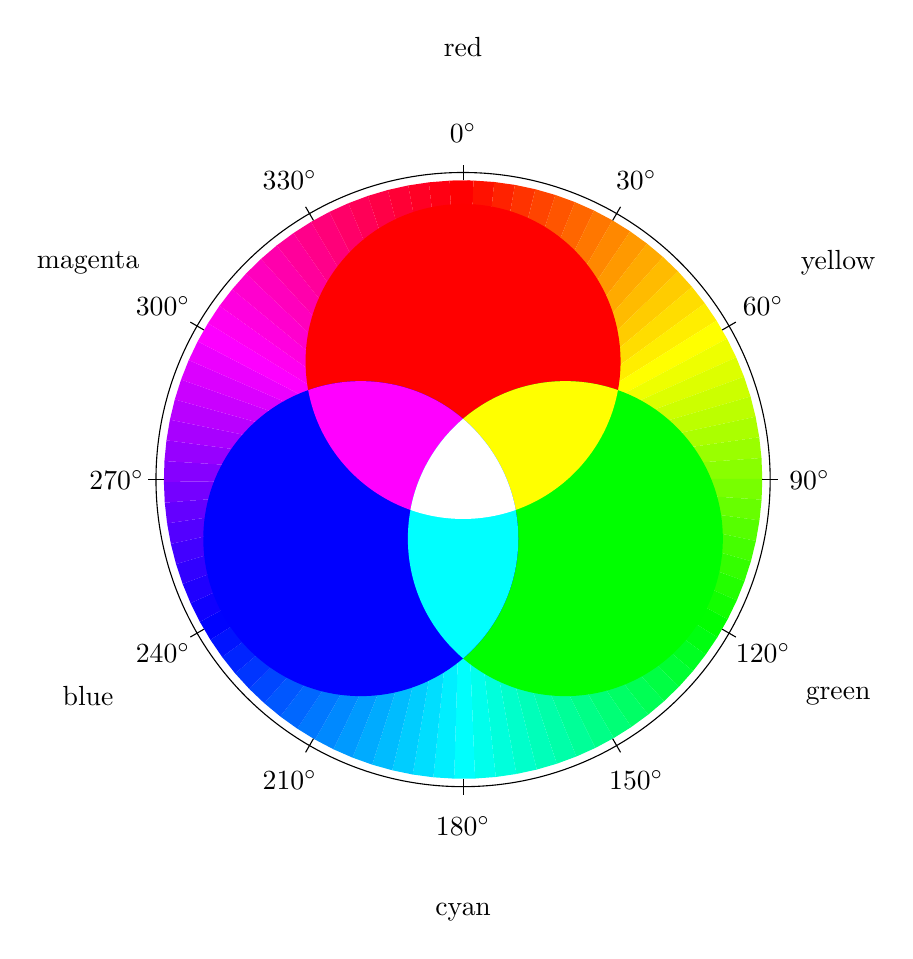
\begin{tikzpicture}
% Create the background in the circle, by drawing several slices
% each with a constant color given by the angle (which is converted
% to a color usin the hue, saturation and brightness color space).
\foreach \x in {0,0.0111,...,1} {
    \definecolor{currentcolor}{hsb}{\x, 1, 1}
    \draw[draw=none, fill=currentcolor]
        (-360*\x+88:2) -- (-360*\x+88:3.8)
        -- (-360*\x+92:3.8) -- (-360*\x+92:2) -- cycle;
}

% On top of the background draw three spotlights of the primary colors
% red, green and blue (they are primary in an additive colorspace where
% light are mixed)
\draw [draw=none, fill=red] (90:1.5) circle (2cm);
\draw [draw=none, fill=green] (-30:1.5) circle (2cm);
\draw [draw=none, fill=blue] (210:1.5) circle (2cm);

% Draw areas where two of the three primary colors are overlapping.
% These areas are the secondary colors yellow, cyan and magenta.
\begin{scope} % red + green = yellow
    \clip (90:1.5) circle(2cm);
    \draw [draw=none, fill=yellow] (-30:1.5) circle (2cm);
\end{scope} % blue + red = magenta
\begin{scope}
    \clip (210:1.5) circle(2cm);
    \draw [draw=none, fill=magenta] (90:1.5) circle (2cm);
\end{scope}
\begin{scope} % green + blue = cyan
    \clip (-30:1.5) circle(2cm);
    \draw [draw=none, fill=cyan] (210:1.5) circle (2cm);
\end{scope}

% Draw the center area which consists of all the primary colors.
\begin{scope} % red + green + blue = white
    \clip (90:1.5) circle(2cm);
    \clip (210:1.5) circle(2cm);
    \draw [draw=none, fill=white] (-30:1.5) circle (2cm);   
\end{scope}

% Draw a circle with markings along the perimeter, indicating which angles
% the hue function connects to certain colors.
\draw (0, 0) circle (3.9cm);
\foreach \x  in {0, 30, ..., 330}
    \draw (-\x+90:3.8) -- (-\x+90:4.0) (-\x+90:4.4) node {$\x^\circ$};

% Add labels with names of the primary and secondary colors.
\foreach \x/\text in {0/red, 60/yellow, 120/green, 180/cyan, 240/blue, 300/magenta}
    \draw (-\x+90:5.5) node {\text};
\end{tikzpicture}


\end{document}
